%!TEX root = ../thesis.tex
\documentclass[../thesis]{subfiles}

\begin{document}
	\section{Results}
	\label{sec:multicore:results}

	\tdg{Rebuçados e methodology}
	Performance measurements are required to verify and quantify the improvements from using the block method over the point one and to properly compare the algorithms for the two presented strategies. This section presents the results obtained for these algorithms with tests running in a single node of the 701 group in the \search\footnote{\url{http://search.di.uminho.pt}} cluster. In addition to what was described in \cref{sec:case:method}, the methodology for these tests also included power-of-two equivalent dimensions (2048, 4096 and 8192). A block dimension of 64 was experimentally found to be the most efficient.

	\tdg{OS and hardware}
	Nodes in this group run Linux CentOS 6.2 with two 8-core \intel\xeon E5-2650 processors and 64GB of shared DRAM (\numa). Each of its processors runs at a clock frequency of 2.00 GHz and has hardware support for 16 simultaneous threads with \intel Hyper-Threading. Further information regarding the hardware in these nodes is shown in \cref{tab:search:701}.

	\tdg{compiler and libraries}
	Tests were built using \intel Composer XE 2011 (compiled with \icpc 12.0.2 and linked with \intel\mkl, for optimized \blas and \lapack) and Armadillo C++ Linear Algebra library (version 3.800.2).

	\begin{table}[p]
		\begin{center}
			\begin{tabular}{lr}
				\hline
				Clock frequency & 2.00 GHz \\
				Cores & 8 \\
				SIMD width & 256-bit (\avx) \\
				Memory size & 64 GB \\
				\hline
				Peak DP FLOPs & 128 GigaFLOP/s \\
				Peak Memory Bandwidth & 51.2 GB/s \\ 
				\hline
			\end{tabular}
		\end{center}
		\caption{Hardware details for \search group 701 nodes. Further information available in \cite{Intel:Xeon:e5_2650,Intel:Xeon:e5_2600}.}
		\label{tab:search:701}
	\end{table}

	\Cref{fig:multicore:point:row:times} shows the execution times obtained for the point method with the row strategy. Preliminary tests with the column strategy showed identical results. It is clear that these strategies does not scale at all, unlike what happens with the diagonal strategy (\cref{fig:multicore:point:diagonal:times}), which reaches its maximum performance when using all the hardware supported threads.

	\begin{figure}[hp]
		\begin{center}
			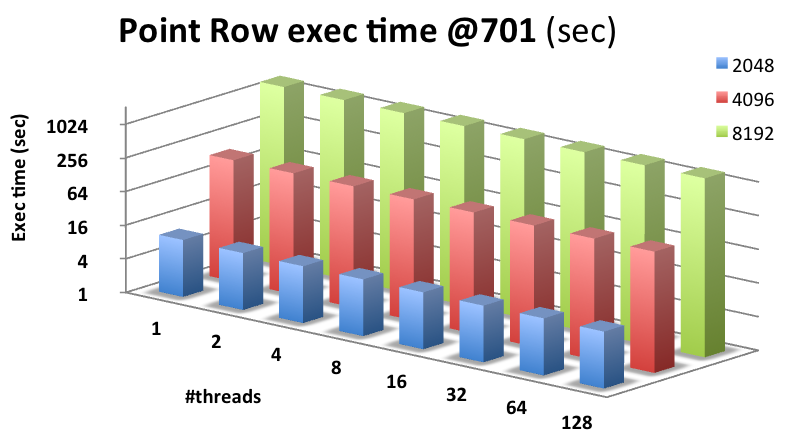
\includegraphics[width=0.9\textwidth]{assets/images/multicore/point-row.png}
		\end{center}
		\caption{Execution times for point method and row strategy}
		\label{fig:multicore:point:row:times}
	\end{figure}

	\begin{figure}[hp]
		\begin{center}
			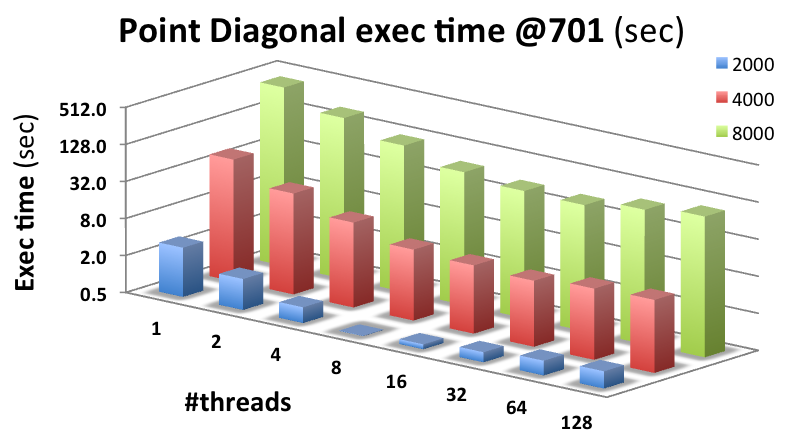
\includegraphics[width=0.9\textwidth]{assets/images/multicore/point-diagonal.png}
		\end{center}
		\caption{Execution times for point method and diagonal strategy}
		\label{fig:multicore:point:diagonal:times}
	\end{figure}

	The block method (\cref{fig:multicore:block:diagonal:times}) also scales well, with the minimum execution time being reached when using 32 threads (the 16 cores with Hyper-Threading). \Cref{fig:multicore:sensitivity} shows that the block method not only is faster than the point method, it is also less sensitive to small variations in the matrix size.

	\begin{figure}[hp]
		\begin{center}
			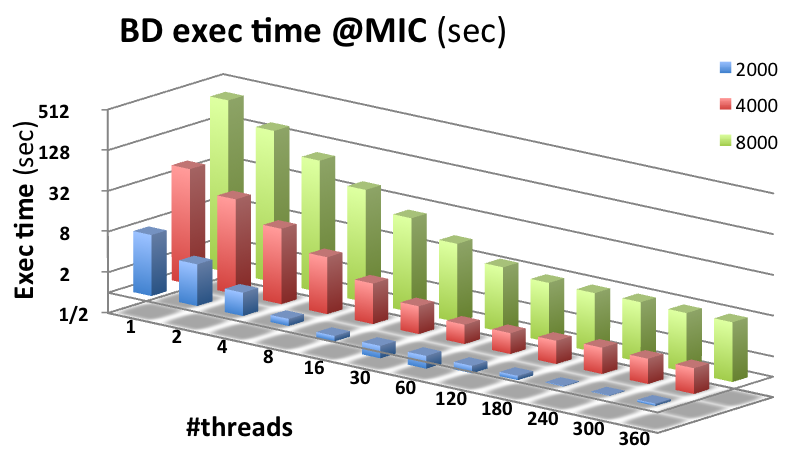
\includegraphics[width=0.9\textwidth]{assets/images/multicore/block-diagonal.png}
		\end{center}
		\caption{Execution times for block method and diagonal strategy}
		\label{fig:multicore:block:diagonal:times}
	\end{figure}

	\begin{figure}[hp]
		\begin{center}
			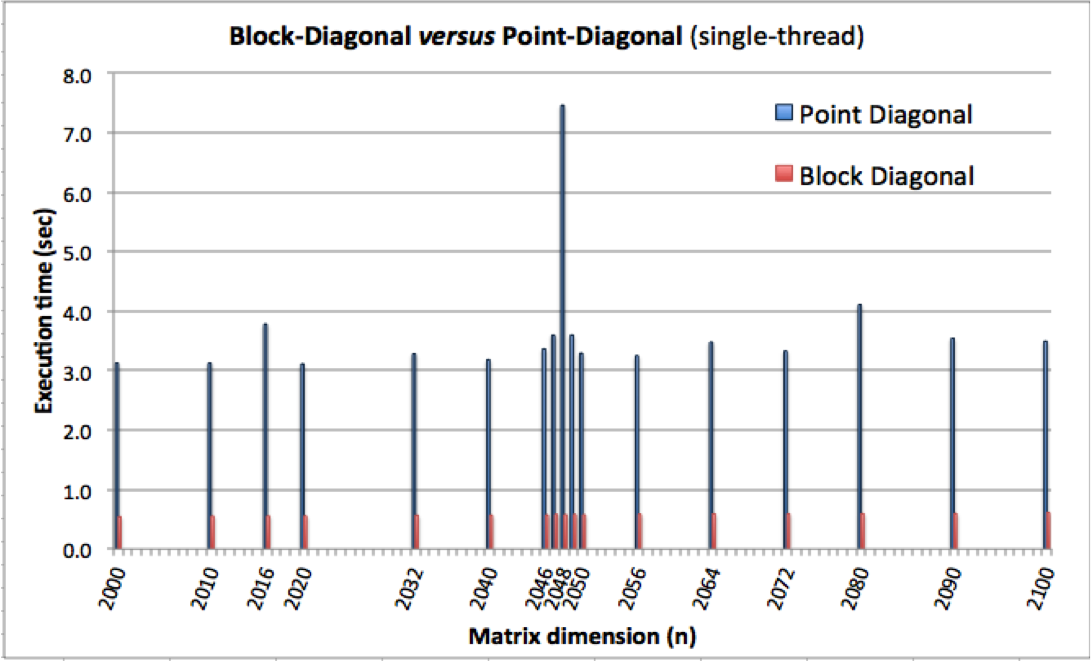
\includegraphics[width=0.9\textwidth]{assets/images/multicore/matrix-variations.png}
		\end{center}
		\caption{Execution time sensitivity for both point and block methods, using diagonal strategy}
		\label{fig:multicore:sensitivity}
	\end{figure}

	\Cref{fig:multicore:block:diagonal:speedup:accumulated} shows the speedup achieved only from blocking when using the diagonal strategy. This speedup is better noticed when using only one thread, since both strategies scale well. The accumulated speedup from both blocking and multithreading shows highly significant speedups, which are even greater when using special specific matrix sizes (\cref{fig:multicore:block:diagonal:speedup:accumulated:strange}).

	\begin{figure}[hp]
		\begin{center}
			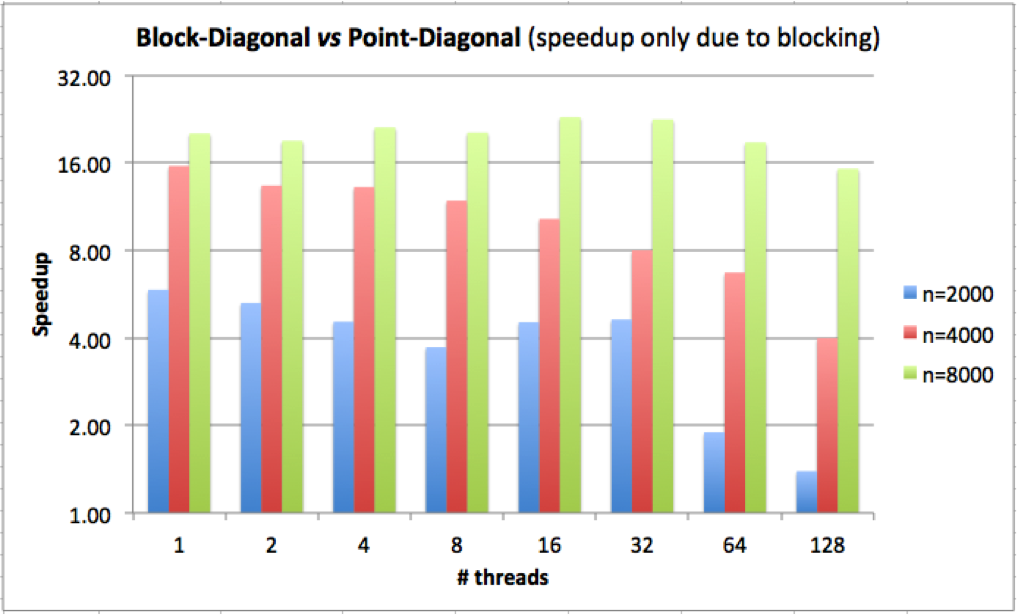
\includegraphics[width=0.9\textwidth]{assets/images/multicore/diagonal-speedup.png}
		\end{center}
		\caption{Speedups achieved with blocking for diagonal strategy}
		\label{fig:multicore:block:diagonal:speedup}
	\end{figure}

	\begin{figure}[hp]
		\begin{center}
			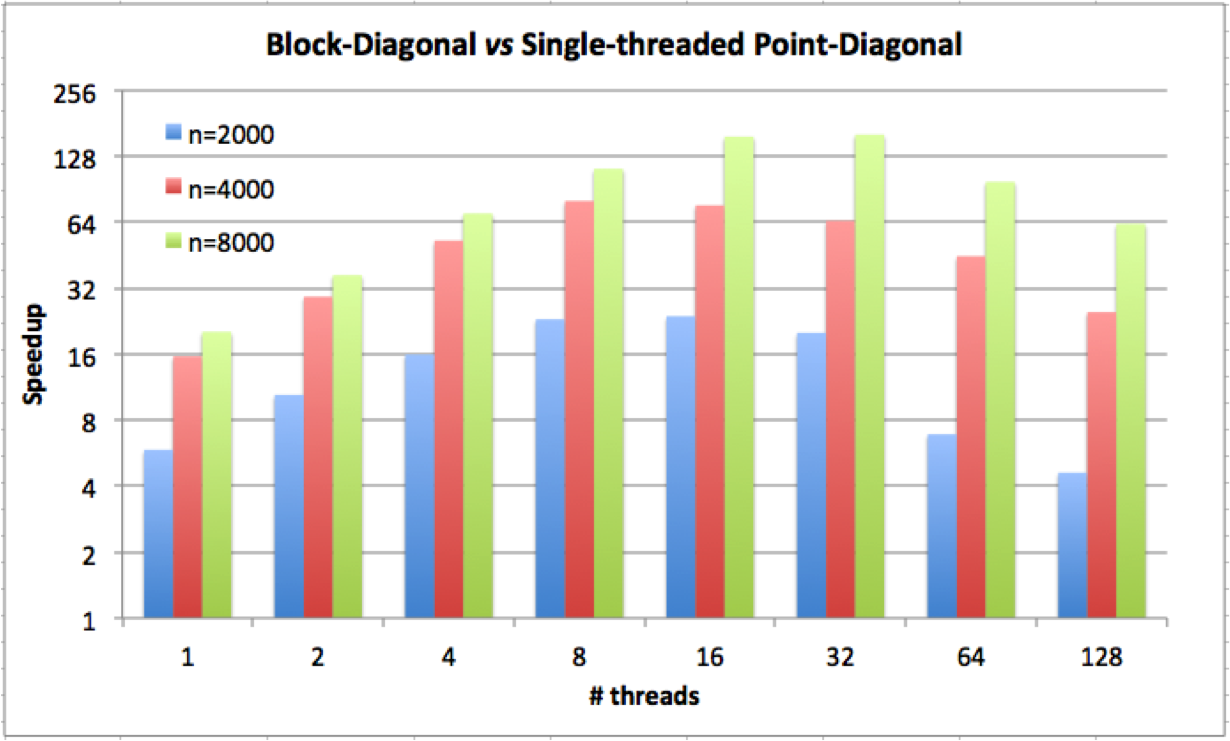
\includegraphics[width=0.9\textwidth]{assets/images/multicore/diagonal-block-stpoint-speedup.png}
		\end{center}
		\caption{Accumulated speedup achieved with blocking for diagonal strategy}
		\label{fig:multicore:block:diagonal:speedup:accumulated}
	\end{figure}

	\begin{figure}[hp]
		\begin{center}
			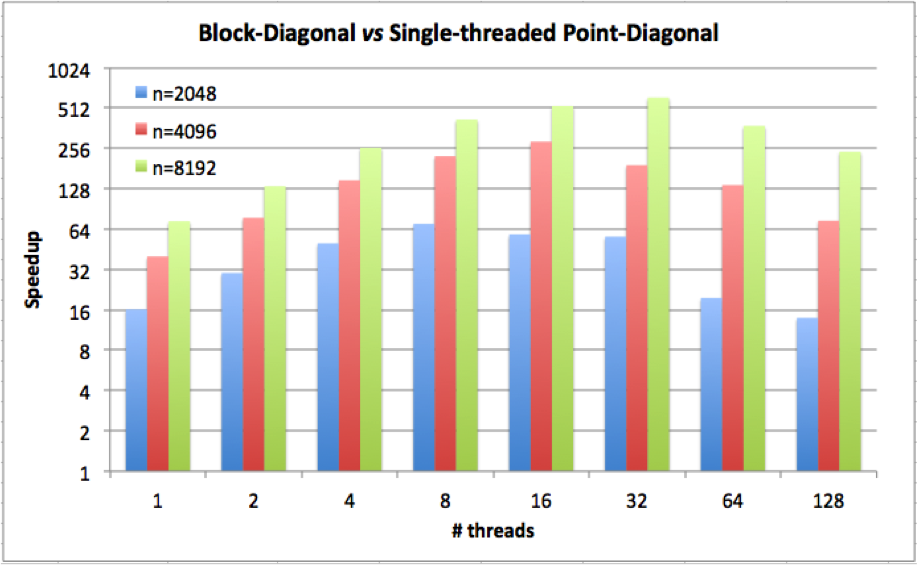
\includegraphics[width=0.9\textwidth]{assets/images/multicore/diagonal-block-stpoint-speedup-strange.png}
		\end{center}
		\caption{Accumulated speedups achieved with blocking for diagonal strategy (power of 2 sizes)}
		\label{fig:multicore:block:diagonal:speedup:accumulated:strange}
	\end{figure}
\end{document}
